\documentclass[11pt]{exam}
% \printanswers

\usepackage{examJF}
\hypersetup{colorlinks,
    linkcolor={upc},
    linktoc=all,
}
\renewcommand\cfttoctitlefont{\normalfont\Large\bfseries\color{upc}}
\renewcommand\cftsecpagefont{\color{upc}}
\renewcommand\cftsecleader{\color{upc}\cftdotfill{\cftsecdotsep}}
\renewcommand\cftsubsecpagefont{\color{upc}}
\renewcommand\cftsubsecleader{\color{upc}\cftdotfill{\cftsubsecdotsep}}
\renewcommand\cftsubsubsecpagefont{\color{upc}}
\renewcommand\cftsubsubsecleader{\color{upc}\cftdotfill{\cftsubsecdotsep}}

%% SECTION AND SUBSECTION TITLE FORMATTING (using examJF's 'upc' color)
\titleformat{\section}
{\normalfont\LARGE\bfseries\color{upc}} % Format for the whole section title line
{\color{upc}\thesection} % Format for the section number
{1em} % Horizontal space between number and title
{} % Code before the title text
\titleformat{\subsection}
{\normalfont\Large\bfseries\color{upc}} % Format for the whole subsection title line
{\color{upc}\thesubsection} % Format for the subsection number
{1em} % Horizontal space between number and title
{} % Code before the title text
\titleformat{\subsubsection}
{\normalfont\large\bfseries\color{upc}} % Format for the whole subsubsection title line
{\color{upc}\thesubsubsection} % Format for the subsubsection number
{1em} % Horizontal space between number and title
{} % Code before the title text

% FOOTER
\footer{\footnotesize Data Analysis Final Project Instructions}
{}
{\footnotesize Page \thepage\ of \numpages}

\begin{document}
    %% FIRST PAGE HEADER
    {\sffamily\color{upc}\noindent\rule{\textwidth}{1.5pt}\\[2mm]
        \begin{minipage}[c]{.18\textwidth}
            \includesvg[width=0.94\textwidth]{./figures/UPC.svg} % Make sure UPC.svg is available
        \end{minipage}
        \hfill
        \begin{minipage}[c]{.6\textwidth}
            \begin{center}
                \vspace*{1mm}{\Large Final Project\\[2mm]\textbf{Data Analysis in Rehabilitation}}\\[3mm]
                {\large Prof. Joan F. Alonso}\\[3mm]
            \end{center}
        \end{minipage}
        \hfill
        \fcolorbox{upc}{upc}{
            \begin{minipage}[c]{.16\textwidth}
                \vspace*{1mm}
                \noindent
                \centering{\\[1mm]{\color{white}\footnotesize Master in\\\textbf{Neuroengineering\\and\\Rehabilitation}\\[1.5mm]{\large 2024/25}}}
                \vspace*{1mm}
            \end{minipage}
        }\\[2mm]
        \noindent\rule{\textwidth}{1.5pt}
    }

    \tableofcontents % Generate a table of contents
    \thispagestyle{empty}
    \setcounter{page}{0}
    \newpage

    % Reset link color for the main document content if desired, or keep as defined above
        \hypersetup{
        linkcolor={FireBrick},
        citecolor={FireBrick},
        urlcolor={FireBrick}
    }

    %% DESCRIPTION
    \section{Introduction and Aim}
    \subsection{Some context}
    Welcome to the integrative data analysis project! Over the next weeks, we will embark on a journey into the field of Brain-Computer Interfaces (BCIs). We will analyse real electroencephalography (EEG) data recorded from volunteers performing motor imagery tasks. Specifically, volunteers imagined moving either their left or their right hand, or they remained in a relaxed state (no movement).

    We will start with raw data, navigate the challenges of biological signal processing, explore feature engineering techniques, and apply machine learning models to decode the brain's intentions. This project provides hands-on experience with a complete data analysis workflow in a challenging and exciting application domain.

    In the \emph{Human-Machine Interfaces (HMI)} course we have already explored the decoding of upper-limb movements using the database described in \href{https://doi.org/10.1371/journal.pone.0182578}{\myul{P. Ofner et al., 2017}}. Specifically, we now know how to:
    \begin{itemize}
        \item \textbf{Band-pass filter EEG signals} and identify bad channels and artefacts.
        \item \textbf{Select usable trials} using trimmed normalisation.
        \item \textbf{Re-reference} signals (common average, Laplacian, etc.).
        \item \textbf{Assess movement execution} on the EEG signals by event-related de/synchronisation (ERD/ERS) and slow cortical potentials (SCP).
        \item \textbf{Represent topographic maps} to check the channels where these potentials are best observed.
    \end{itemize}

    Therefore, in this project we will use this knowledge to decipher the movement imagined by a person.

    \subsection{Key points}

    \begin{itemize}
        \item \textbf{Primary aim of the project}\\To design, implement, and evaluate a machine learning pipeline capable of accurately classifying different motor imagery states (left-hand, right-hand imagery, no imagery) based solely on the recorded EEG signals.
        \item \textbf{Duration}\\6 \textonehalf~weeks (from 28th April to 11th June, 2025)
        \item \textbf{Group Size}\\4 students
        \item \textbf{Grading}\\~
        \SI{70}{\percent} Report, \SI{30}{\percent} Presentation.\\ Details on the deliverables are in \Cref{subsec:report}. The rubrics used to assess the project are available in \Cref{ann:projectrubric} and \Cref{ann:presentationrubric}.
    \end{itemize}


    \newpage
    \section{Project Phases and Tasks}
    \subsection{Proposed Planning}

    \begin{ganttchart}[
        % --- Font Size Options ---
        title label font=\small,  % Adjust size for calendar titles
        bar label font=\footnotesize, % Adjust size for task labels
        group label font=\small, % Adjust size for group labels
        milestone label font=\footnotesize, % Adjust size for milestones
        % --- Indentation Option ---
        bar label node/.append style={xshift=1em}, % Indent bar labels
        % --- Other Options ---
        x unit=2.35mm,
        y unit chart=4.5mm,
        time slot unit=day,
        time slot format=isodate,
        vgrid,
        hgrid,
        bar label node/.append style={text width=6cm, align=left},
        group label node/.append style={text width=6cm, align=left}
        ]{2025-04-28}{2025-06-15} % Ensure these dates are correct


        % Title Setup - shows months & weeks
        \gantttitlecalendar{month=shortname, week} \\

        % --- Phase 1: Data Understanding (Apr 28 - May 3) ---
        \ganttgroup[group/.append style={fill=RoyalBlue!90}]{Phase 1: Exploratory Data Analysis}{2025-04-28}{2025-05-03} \\
        \ganttbar[bar/.append style={fill=RoyalBlue!60}]{Task 1.1: Loading and Exploration}{2025-04-28}{2025-04-29} \\
        \ganttbar[bar/.append style={fill=RoyalBlue!45}]{Task 1.2: Data Cleansing}{2025-04-29}{2025-04-29} \\
        \ganttbar[bar/.append style={fill=RoyalBlue!30}]{Task 1.3: Preprocessing}{2025-04-30}{2025-05-01} \\
        \ganttbar[bar/.append style={fill=RoyalBlue!20}]{Task 1.4: Visualisation}{2025-05-02}{2025-05-03} \\

        % --- Phase 2: Feature Engineering (May 4 - May 18) ---
        \ganttgroup[group/.append style={fill=ForestGreen!90}]{Phase 2: Feature Engineering}{2025-05-04}{2025-05-18} \\
        \ganttbar[bar/.append style={fill=ForestGreen!70}]{Task 2.1: Spectral, ERD/ERS}{2025-05-04}{2025-05-06} \\
        \ganttbar[bar/.append style={fill=ForestGreen!60}]{Task 2.2: Time, MRCP}{2025-05-07}{2025-05-08} \\
        \ganttbar[bar/.append style={fill=ForestGreen!50}]{Task 2.3: Common Spatial Patterns}{2025-05-09}{2025-05-12} \\
        \ganttbar[bar/.append style={fill=ForestGreen!40}]{Task 2.4: Other Features}{2025-05-12}{2025-05-13} \\
        \ganttbar[bar/.append style={fill=ForestGreen!30}]{Task 2.5: Feature Selection/Extraction}{2025-05-13}{2025-05-16} \\
        \ganttbar[bar/.append style={fill=ForestGreen!20}]{Task 2.6: Standardisation}{2025-05-17}{2025-05-18} \\

        % --- Phase 3: Model Training (May 16 - Jun 1) ---
        \ganttgroup[group/.append style={fill=DarkOrange}]{Phase 3: Model Training}{2025-05-16}{2025-06-01} \\
        \ganttbar[bar/.append style={fill=DarkOrange!60}]{Task 3.1: Model Selection}{2025-05-16}{2025-05-22} \\
        \ganttbar[bar/.append style={fill=DarkOrange!50}]{Task 3.2: Training Pipeline}{2025-05-21}{2025-05-25} \\
        \ganttbar[bar/.append style={fill=DarkOrange!40}]{Task 3.3: Validation}{2025-05-25}{2025-05-29} \\
        \ganttbar[bar/.append style={fill=DarkOrange!30}]{Task 3.4: Performance Metrics}{2025-05-29}{2025-06-01} \\

        % --- Phase 4: Assessment & Reporting (May 1 - Jun 11) ---
        \ganttgroup[group/.append style={fill=FireBrick!90}]{Phase 4: Assessment and Report}{2025-05-01}{2025-06-11} \\ % Changed & to and
        \ganttbar[bar/.append style={fill=FireBrick!60}]{Task 4.1: Offline Testing}{2025-06-02}{2025-06-03} \\
        \ganttbar[bar/.append style={fill=FireBrick!50}]{Task 4.2: Analysis and Discussion}{2025-06-04}{2025-06-06} \\ % Changed & to and
        \ganttbar[bar/.append style={fill=FireBrick!40}]{Task 4.3: Report Preparation}{2025-05-01}{2025-06-10} \\
        \ganttmilestone[milestone/.append style={fill=FireBrick}]{Deliver Report (ATENEA, 11th June)}{2025-06-11} \\
        \ganttbar[bar/.append style={fill=FireBrick!30}]{Task 4.4: Presentation Preparation}{2025-06-04}{2025-06-11} \\
        \ganttmilestone[milestone/.append style={fill=FireBrick}]{Presentation (Room 4.2, 12th June)}{2025-06-12}

    \end{ganttchart}

    \subsection{Phase 1: Exploratory Data Analysis}
    \begin{itemize}
        \item \textbf{Objective:} Familiarise yourselves with the EEG dataset and prepare it for analysis.
        \item \textbf{Tasks:}
        \begin{itemize}
            \item \textbf{Data Loading and Exploration:} Load \href{https://drive.google.com/drive/folders/1b7Uo\_FO52\_-f4F-DbzYgpeiylx90f\_-n}{\myul{the provided EEG datasets (in EEGLab \texttt{.mat} format)}}. Understand the data structure, channel layout (based on the 16-channel OpenBCI setup), and event markers indicating the different imagery tasks.

            \Cref{annex:database} describes the contents and format of the shared files.

            \item \textbf{Data Cleansing:} Identify and handle potential issues like noise, artefacts (e.g., blinks, ocular movements, muscular activity from the head and neck), and bad channels. Decide on appropriate strategies for correction and/or removal.
            \item \textbf{Preprocessing:} Apply necessary preprocessing steps such as filtering (e.g., bandpass filtering to isolate relevant frequency bands), referencing, and epoching (segmenting the data into trials based on task markers).
            \item \textbf{Data Visualisation:} Create informative visualisations (e.g., time series plots, power spectral density plots, topographic plots) to understand the characteristics of the EEG signals during different tasks and to guide preprocessing choices.
        \end{itemize}
        \item \textbf{Comments:} It may be easier to do this in MATLAB, reusing code developed in \emph{HMI}.
    \end{itemize}

    \begin{figure}[htbp]
        \centering
        \Acrobatmenu{GoBack}{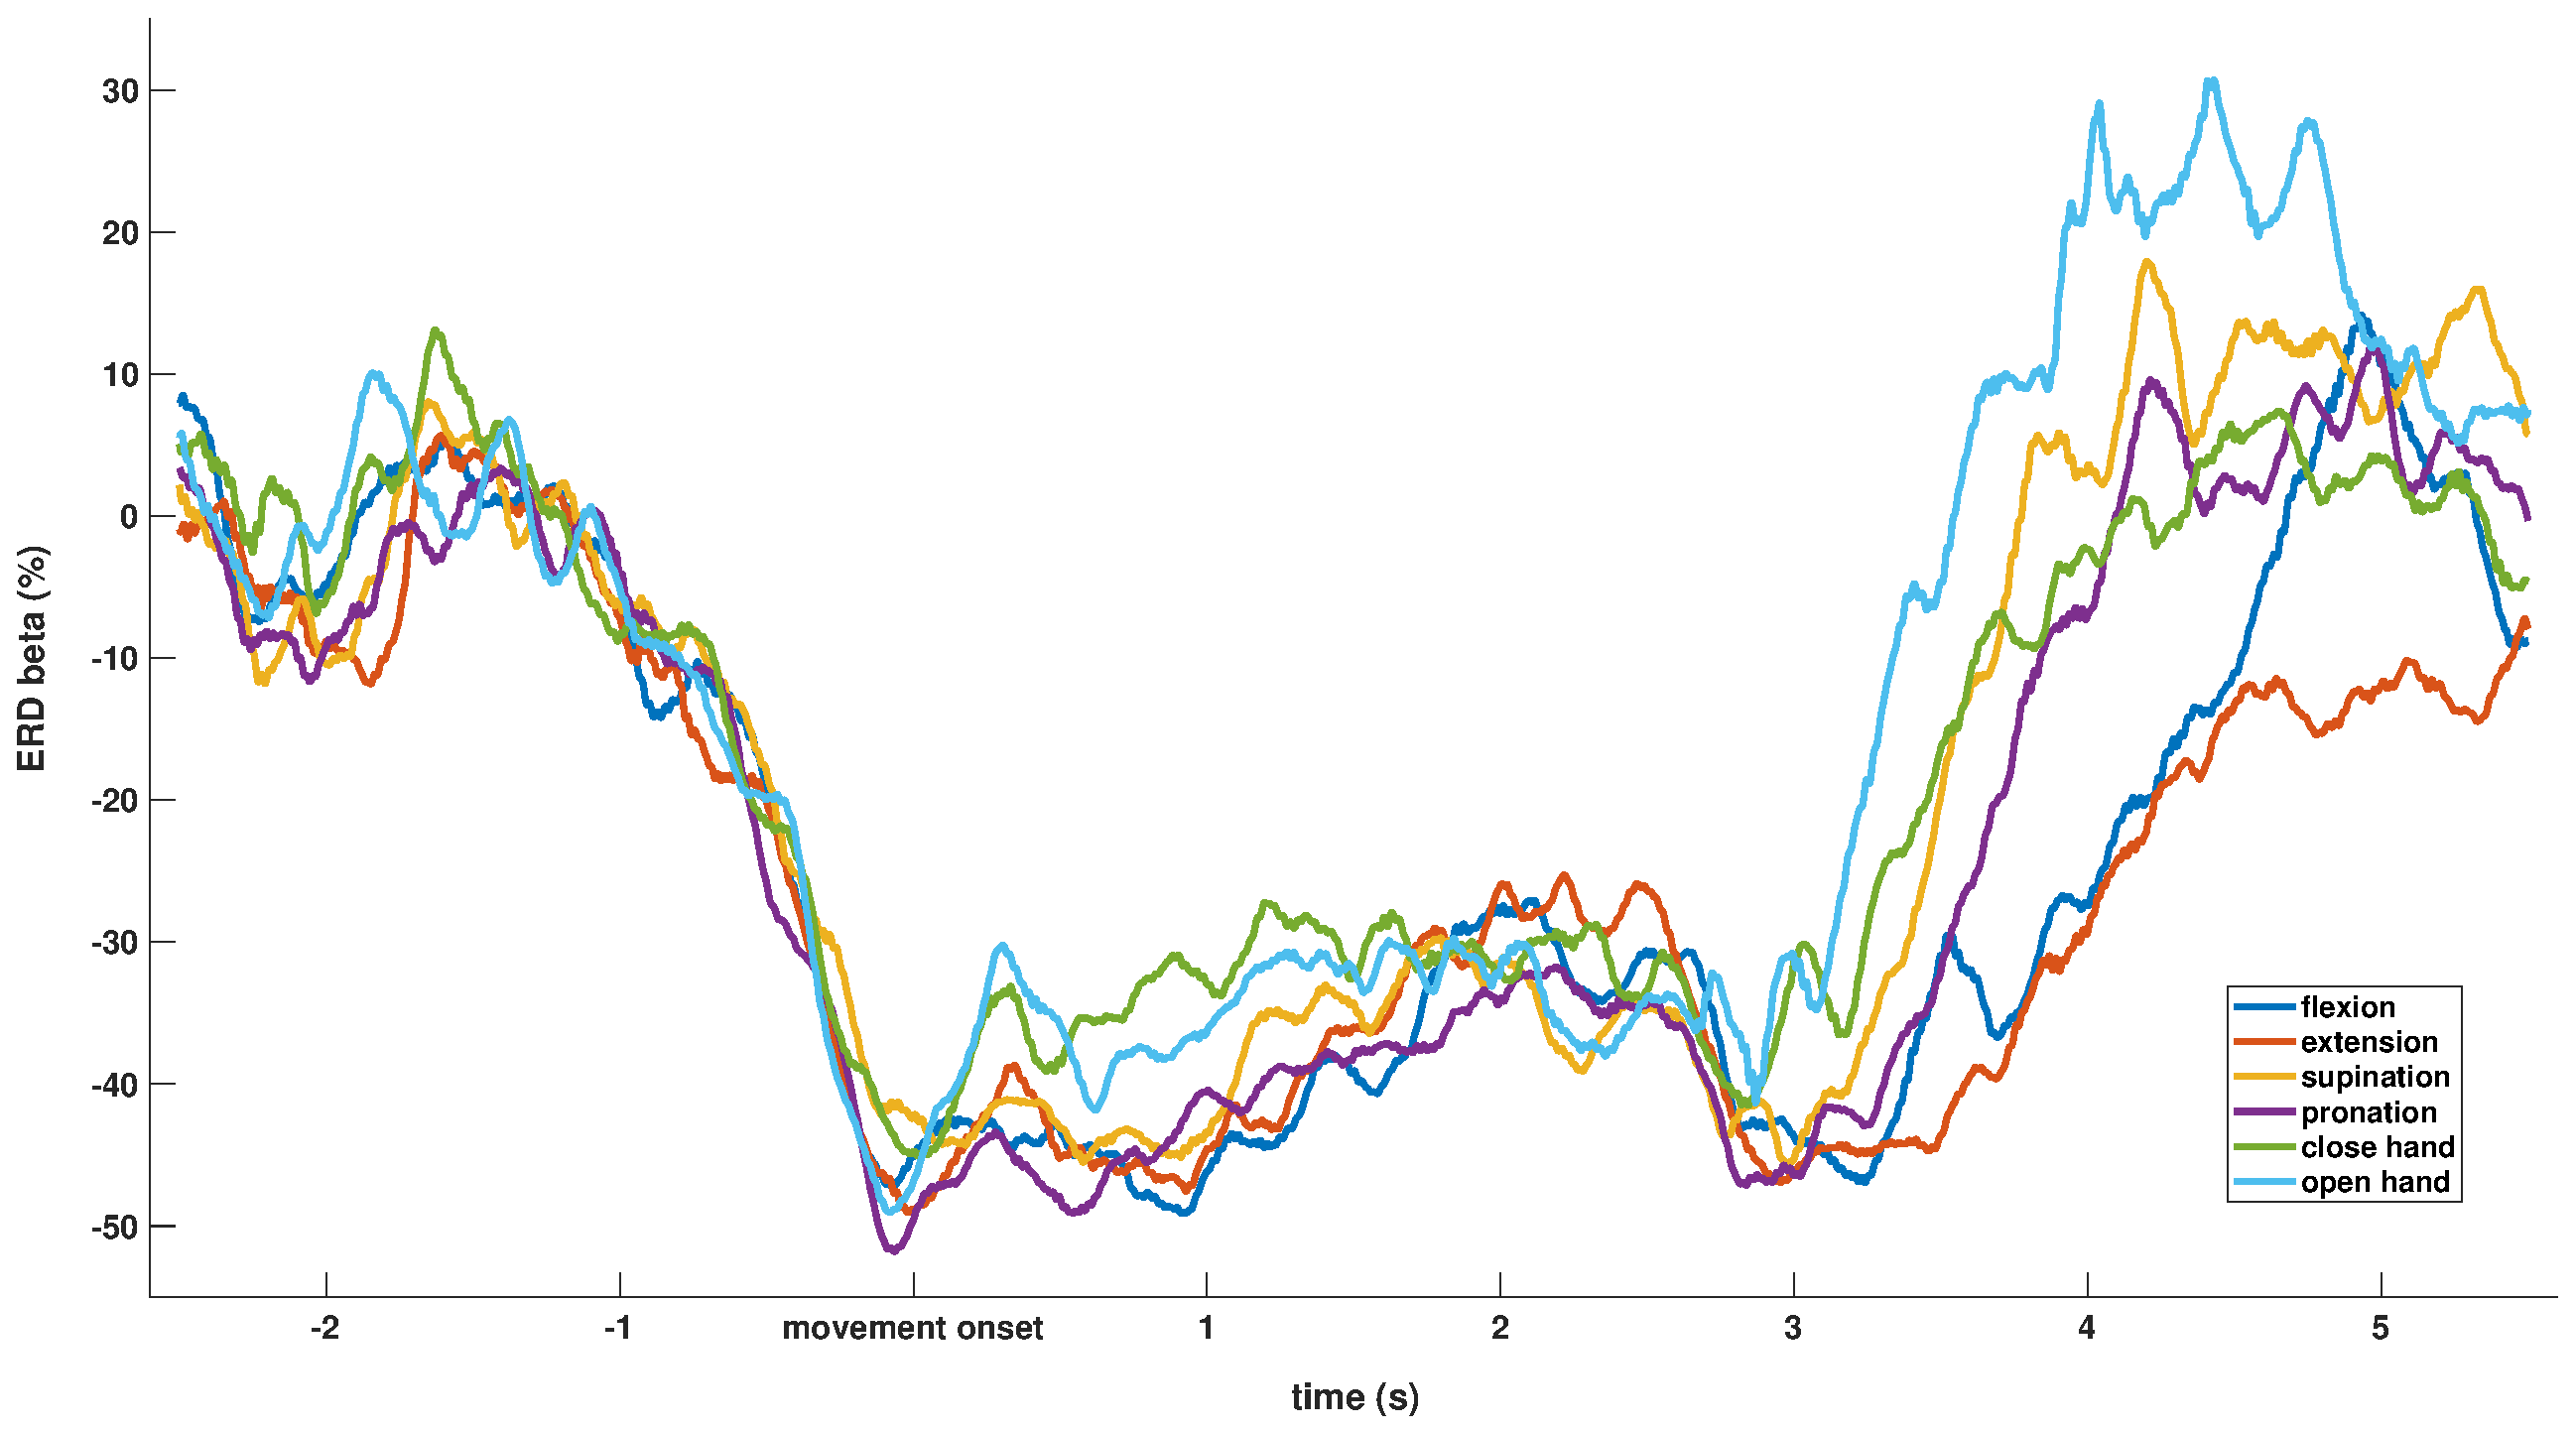
\includegraphics[width=14cm]{./figures/ERDbeta_av_2022.eps}} % Ensure figure path is correct
        \caption{Grand-average ERD/ERS potentials obtained in the \(\beta\) band for\\the movements in \href{https://doi.org/10.1371/journal.pone.0182578}{\myul{P. Ofner et al., 2017}}.Image by S. Romero.}
        \label{fig:ERD}
    \end{figure}

    \smallskip % Add some vertical space between figures
    \begin{figure}[htbp]
        \centering
        \Acrobatmenu{GoBack}{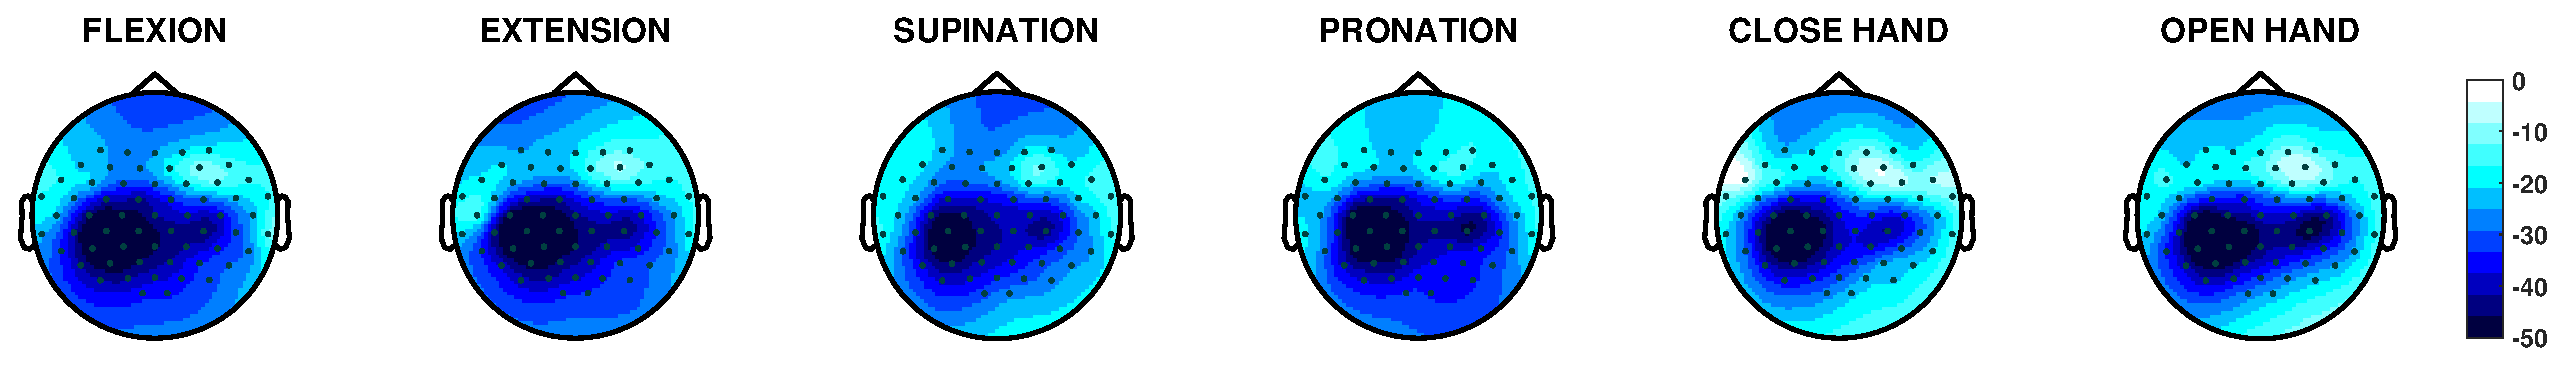
\includegraphics[width=17.5cm]{./figures/ERDbeta_topography_2022.eps}} % Ensure figure path is correct
        \caption{Grand-average ERD potentials (in \si{\micro\volt}) obtained in the \(\beta\) band at the movement onset,\\for the movements in \href{https://doi.org/10.1371/journal.pone.0182578}{\myul{P. Ofner et al., 2017}}. Image by S. Romero.}
        \label{fig:ERDtopo}
    \end{figure}

    \subsection{Phase 2: Feature Engineering and Selection/Extraction} % Changed & to and
    \begin{itemize}
        \item \textbf{Objective:} Create meaningful features from the preprocessed EEG data that can aid discrimination between the different motor imagery states.
        \item \textbf{Tasks:}
        \begin{itemize}
            \item \textbf{Brainstorming and Feature Engineering:} Explore and implement various feature types relevant to motor imagery EEG, including:
            \begin{itemize}
                \item \textbf{Frequency-based features:} Investigate ERD/ERS patterns, typically observed in the \(\mu\) (\SIrange{8}{13}{\hertz}) and \(\beta\) (\SIrange{14}{30}{\hertz}) bands over motor cortex areas during motor imagery (See \Cref{fig:ERD} and \Cref{fig:ERDtopo}). Calculate band power or related metrics.
                \item \textbf{Time-domain features:} Explore Movement-Related Cortical Potentials (MRCPs), although these are often more prominent in actual movement, investigate if relevant components exist in the imagery data. These potentials are usually best detected when the signal is low-pass filtered (e.g. from \SIrange{0.3}{3}{\hertz}). Keep in mind that slow cortical potentials are best detected around central locations (Cz and neighbouring electrodes), as seen in the maps in \Cref{fig:SCPtopo}.
                \item \textbf{Common Spatial Patterns (CSP):} Implement and utilise CSP, a powerful technique for BCI that finds spatial filters maximising variance between classes. Experiment with the number of patterns/filters. Additional insights on CSP \href{https://doi.org/10.1109/MSP.2008.4408441}{\myul{in this article by B. Blankertz et al. 2007}}.
                \item \textbf{Other potential features} (e.g., statistical measures, connectivity metrics).
            \end{itemize}

            \begin{figure}[htbp]
                \centering
                \Acrobatmenu{GoBack}{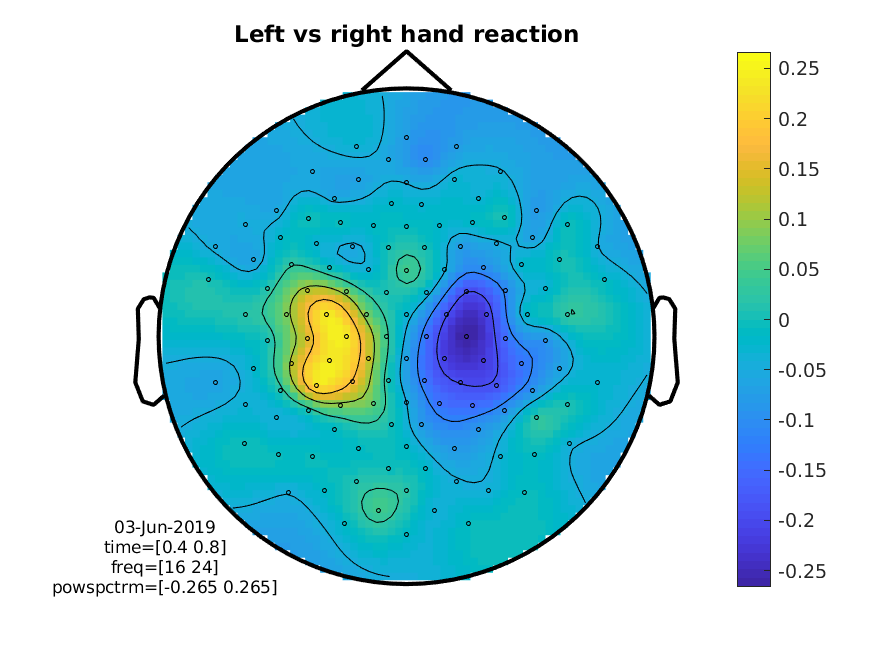
\includegraphics[width=8cm]{./figures/tfr_diff.png}}
                 \caption{Topographic representation of the difference\\in beta power between left and right response. Taken from \href{https://www.fieldtriptoolbox.org/workshop/oslo2019/timefrequency/}{\myul{a FieldTrip tutorial}}}.
            \end{figure}

            \item \textbf{Feature Analysis and Selection/Extraction:} % Changed & to and
            \begin{itemize}
                \item Analyse the discriminative power of individual features or feature sets.
                \item Use techniques like training and validation curves to assess potential overfitting or underfitting with different feature sets.
                \item Evaluate feature redundancy (e.g., using correlation matrices).
                \item Decide whether to use feature selection methods (choosing a subset of the best features) or feature extraction methods (like PCA or potentially using CSP itself as a dimensionality reduction technique). Justify your choices.
            \end{itemize}
            \item \textbf{Standardisation/Normalisation:} Apply appropriate scaling techniques to ensure features are comparable.
        \end{itemize}
        \item \textbf{Comments:}
        \begin{itemize}
            \item The articles by \href{https://doi.org/10.1109/tnsre.2006.875637}{\myul{D. J. McFarland et al., 2005}}
            and by \href{https://doi.org/10.1109/ACCT.2015.72}{\myul{S. Vaid et al., 2015}} can assist in discovering other useful features in BCI systems.
            \item Feature engineering may also be easier in MATLAB, adapting \emph{HMI} codes. CSP can also be calculated easily \href{https://es.mathworks.com/matlabcentral/fileexchange/72204-common-spatial-patterns-csp}{\myul{using MATLAB}}. A Python alternative (\href{https://mne.tools/stable/install/mne_python.html}{\myul{MNE-Python package}}), should you wish to code everything in Python, is also very useful (see \href{https://mne.tools/stable/auto_examples/decoding/decoding_csp_eeg.html}{\myul{example}}).
            \item Below (see pages \pageref{code:MATLAB1} to \pageref{code:MATLAB2}) you can find a basic example of:
            \begin{itemize}
                \item a code structure to process signals and calculate features;
                \item how to use a MATLAB table to store features;
                \item how to export a table to a \texttt{.csv} file.
            \end{itemize}
        \end{itemize}
    \end{itemize}

    \begin{figure}[htbp]
        \centering
        \Acrobatmenu{GoBack}{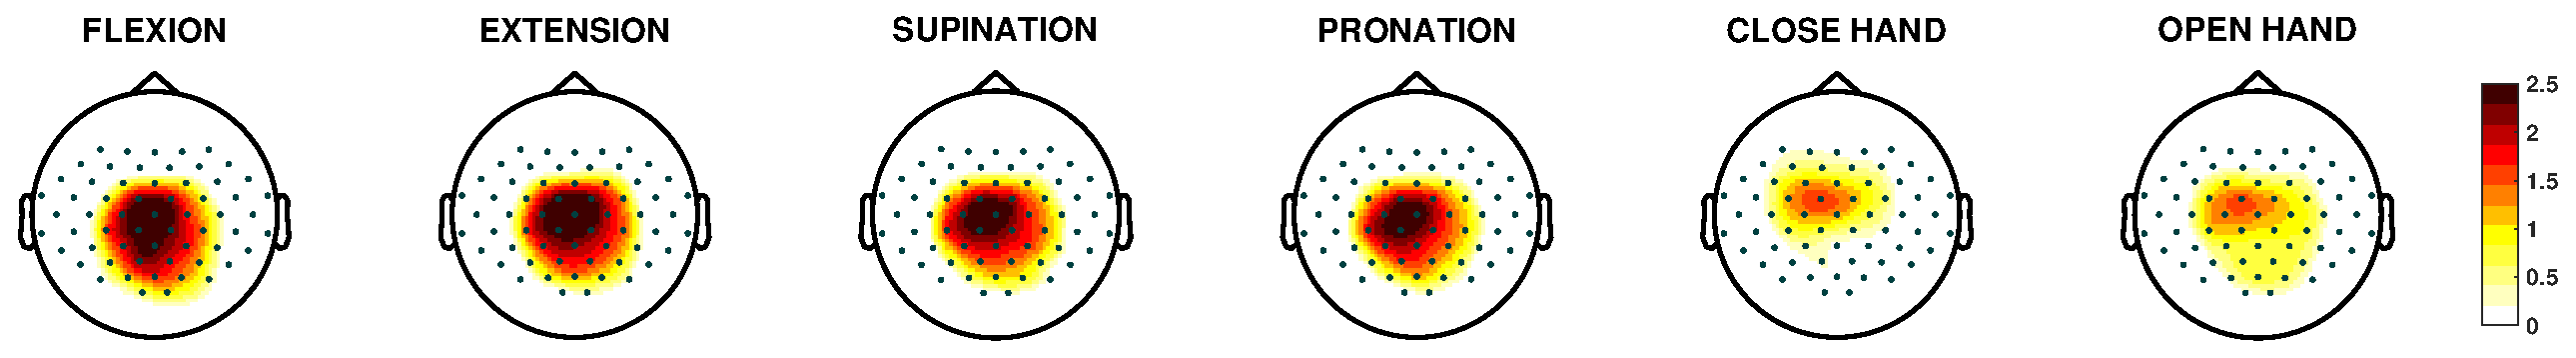
\includegraphics[width=17.5cm]{./figures/SCP_topography_2022.eps}} % Ensure figure path is correct
        \caption{Slow cortical potential topographies for the movements in \href{https://doi.org/10.1371/journal.pone.0182578}{\myul{P. Ofner et al., 2017}}.\\ Maps show the grand-average amplitude in \si{\micro\volt} of a \SI{0.5}{\second} segment selected just before\\the movement onset. Image by S. Romero.}
        \label{fig:SCPtopo}
    \end{figure}


    % MATLAB Code Example
    \label{code:MATLAB1} % Label for cross-referencing page number
    \inputminted[frame=lines,
    framesep=4mm,
    baselinestretch=0.85,
    linenos,
    numbersep=2mm,
    xleftmargin=15mm,
    xrightmargin=15mm,
    label={MATLAB Code to process all trials of a subject},
    style=xcode]
    {matlab}{./codes/example_structure.m} % Ensure code path is correct

    % CSV Export Example
    \label{code:MATLAB2} % Label for cross-referencing page number
    % Removed the outer \begin{center}...\end{center}
    \begin{minipage}[t]{0.4\textwidth} % Keep minipage for layout if needed
        \inputminted[frame=lines,
        framesep=4mm,
        baselinestretch=0.85,
        linenos,
        numbersep=2mm,
        xleftmargin=8mm,
        label={Exported 'features.csv' file},
        style=xcode]
        {text}{./codes/features.csv} % Ensure code path is correct
    \end{minipage}
    % Removed \bigskip here to potentially fix blank page issue

    \subsection{Phase 3: Model Training and Validation} % Changed & to and
    \begin{itemize}
        \item \textbf{Objective:} Train and rigorously evaluate different machine learning models for the classification task.
        \item \textbf{Tasks:}
        \begin{itemize}
            \item \textbf{Model Selection:} Choose at least 2 or 3 different classification algorithms suitable for this type of data (e.g., Linear Discriminant Analysis (LDA), Logistic Regression (LR), k-Nearest Neighbors (KNN), Support Vector Machines (SVM), or even ensemble methods like Random Forests or Gradient Boosting).
            \item \textbf{Training Pipeline:} Develop a clear pipeline that incorporates your chosen preprocessing, feature engineering/selection, and classification steps.
            \item \textbf{Validation:} Implement a robust validation strategy (e.g. hold-out, k-fold cross-validation) to evaluate model performance and tune hyperparameters reliably. Avoid testing on the left-out subject during this phase.
            \item \textbf{Performance Metrics:} Select and calculate appropriate performance metrics (e.g., accuracy, precision, recall, F1-score, confusion matrix) to compare the models effectively.
        \end{itemize}
        \item \textbf{Comments:} In this part you will be using Python (importing \texttt{.csv} files generated by MATLAB), as we have done throughout the course.
        \begin{figure}[htbp]
            \centering
            \Acrobatmenu{GoBack}{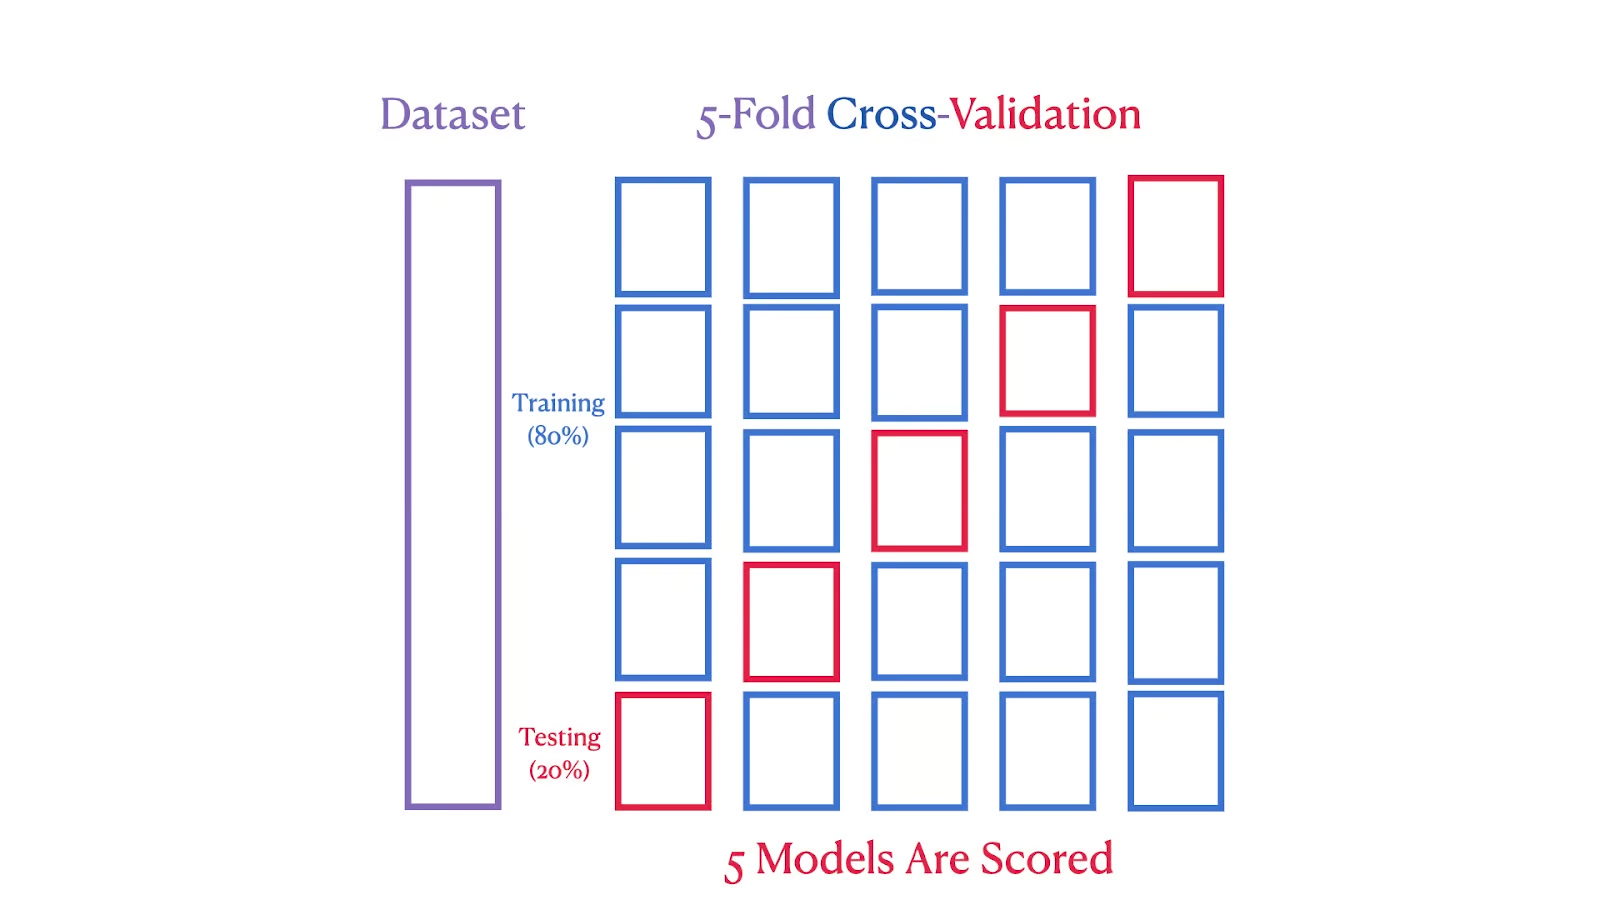
\includegraphics[width=12cm]{./figures/5-fold-CV.png}}
            \caption{5-fold cross-validation scheme. Taken from \href{https://www.datacamp.com/tutorial/k-fold-cross-validation}{\myul{a datacamp.com tutorial}}}.
        \end{figure}

        Model selection will also depend on your feature selection/extraction strategy. For example, if you use a \emph{wrapping} approach and change the model, you may need to run feature selection for each model. If you choose a \emph{filtering} approach, feature selection is model-independent, but less optimised for the chosen model.

        Keep in mind that, in this project, there is no “best” or “correct” way of choosing a validation strategy. You are free to try any alternative:
        \begin{itemize}
            \item All but one subject to train, \textbf{leaving one out} to test each time (selecting the best model as the one with best average performance),
            \item Implement a \textbf{hold-out} strategy by training with some subjects and testing with the rest,
            \item Training a model on each subject, leaving out some data to test each time (\textbf{stratified hold-out}), and then choosing the model also based on average performance.
            \item \textbf{Or something completely different} that you may come up with (perhaps devising an original approach, surprise your instructors!).
            The primary consideration here is to choose a strategy, interpret and understand the results obtained, and propose changes or improvements depending on them.
        \end{itemize}
        Also, take into account that we are dealing with a \textbf{3-class classification problem}, but it can be divided into \textbf{two 2-class classification problems}: rest vs motor imagery and then left vs right. In this case, discuss the suitability of each metric for this potentially imbalanced problem.
    \end{itemize}

    \begin{figure}[htbp]
        \centering
        \Acrobatmenu{GoBack}{\includesvg[width=14cm]{./figures/workflow_with_validation_set.svg}}
        \caption{A good workflow for development and testing. Taken from \href{https://developers.google.com/machine-learning/crash-course/overfitting/dividing-datasets}{\myul{a machine learning course by Google}}.}
    \end{figure}

    \subsection{Phase 4: Final Model Assessment and Reporting}
    \begin{itemize}
        \item \textbf{Objective:} Evaluate your best-performing model(s) on unseen data and prepare your final report and presentation.
        \item \textbf{Tasks:}
        \begin{itemize}
            \item \textbf{Offline Testing:} Apply your final, trained model pipeline(s) to a separate, unseen test dataset (the left-out subject or your own recordings using the same protocol and OpenBCI headset). Report the performance on this dataset.
            \item \textbf{Analysis and Discussion:} Analyse your results, discuss the strengths and weaknesses of your approach, compare the performance of different features and models, and reflect on challenges encountered. Include in the discussion a evaluation of your pipeline in terms of procesing load and response time (both training and applying the model), commenting on its suitability for real-time use. Does anything need to change? How would you make it work on real-time EEG signals?
            \item \textbf{Final Report and Presentation:} Prepare a comprehensive report detailing your entire workflow, methodology, results, and conclusions. Deliver a group presentation summarising your project.
        \end{itemize}
        \item \textbf{Comments:} More details on the deliverables in \Cref{sec:deliverables}.
    \end{itemize}

    \newpage
    \section{Deliverables}
    \label{sec:deliverables}

    \subsection{Outputs of the Project}
    This project is expected to produce three outputs:
    \begin{itemize}
        \item Well-documented code implementing the full analysis pipeline. Predictably, MATLAB and Python code (either code files or Jupyter Notebooks).
        \item A final written report.
        \item A group presentation summarising the project and findings. % British spelling summarising is correct
    \end{itemize}

    These three items will be included in 2 deliverables, described in \Cref{subsec:report} and \Cref{subsec:presentation}.

    \subsection{Final Report}
    \label{subsec:report}
    \subsubsection{Contents}
    Your final report should be a clear, concise, and well-structured document detailing your data analysis project. Please ensure it includes the following sections:

    \begin{itemize}
        \item \textbf{Introduction:}
        \begin{itemize}
            \item Clearly state the problem or research question being addressed.
            \item Explain the motivation and importance of the analysis.
            \item Define the specific objectives of your project.
            \item Briefly outline the report's structure.
        \end{itemize}

        \item \textbf{Data Description:}
        \begin{itemize}
            \item Identify the data source(s).
            \item Provide an overview of the data (variables, size, structure).
            \item Detail all data preprocessing steps (cleaning, handling missing values, transformations, feature engineering) and justify why they were necessary.
        \end{itemize}

        \item \textbf{Methodology:}
        \begin{itemize}
            \item Describe the analytical techniques and models used (e.g., EDA, statistical tests, classification).
            \item Justify your choice of methods based on the project objectives and data characteristics.
            \item Mention key software or libraries used. % British spelling libraries is correct
        \end{itemize}

        \item \textbf{Results:}
        \begin{itemize}
            \item Present your main findings objectively.
            \item \textbf{Crucially:} Include \textbf{meaningful figures and tables} that are clearly labelled (titles, axes, legends) and have descriptive captions explaining what they show. % Corrected labelled
            \item Reference all figures and tables within the text (e.g., "Figure 1 shows...").
            \item Provide \textbf{accompanying comments} that explain the key insights derived from each figure and table. Do not just present visuals without explanation.
        \end{itemize}

        \item \textbf{Discussion:}
        \begin{itemize}
            \item \textbf{Interpret} the results – explain what they mean in the context of your problem/question.
            \item Relate your findings back to the initial objectives.
            \item Discuss any limitations of your data or methodology.
            \item Consider the implications or potential applications of your findings.
        \end{itemize}

        \item \textbf{Conclusion:}
        \begin{itemize}
            \item Summarise the primary conclusions drawn from your analysis. % Corrected Summarise
            \item Directly answer the initial research question based on your findings.
            \item Optionally, suggest potential areas for future work.
        \end{itemize}

        \item \textbf{References:}
        \begin{itemize}
            \item List all cited sources (datasets, articles, tools) using a consistent citation style.
        \end{itemize}

        \item \textbf{Annexes:} % Use Annexes plural here
        \begin{itemize}
            \item Include supplementary material (e.g., code snippets, extra plots) if it supports the main report but is too detailed for the body.
        \end{itemize}
    \end{itemize}

    \textbf{Overall Expectation:} The report should demonstrate a clear understanding of the problem, thoughtful application of data analysis techniques, and the ability to derive and communicate meaningful conclusions supported by well-presented evidence (figures, tables, and insightful commentary).

    \subsubsection{Delivery}
    \begin{itemize}
        \item The report is expected to be delivered \href{https://atenea.upc.edu/mod/assign/view.php?id=4865448}{\myul{via ATENEA}} \textbf{before the end of 11th June}.
        \item The document should be \textbf{one PDF document}. Additional files or information that cannot be included as annexes (such as \texttt{.csv} files or \texttt{.ipynb} notebooks), will be added in an \textbf{additional \texttt{.zip} file}. The \textbf{maximum allowed size} for each file is $\SI{\mathbf{200}}{\mathbf{\mega\byte}}$. % British spelling allowed is correct
        \item \textbf{Do not include code as screenshots or images, code must be text that can be copied and pasted}. The use of \LaTeX\ is highly recommended. You may use this document as a reference if you are unsure where to start; the \LaTeX~source is available \href{https://github.com/joanfrancesc/Data-Analysis-Project}{\myul{here}}.

        \begin{figure}[htbp]
            \centering
            \Acrobatmenu{GoBack}{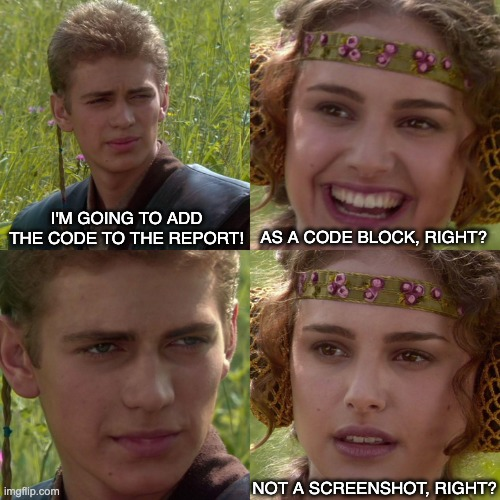
\includegraphics[width=8cm]{./figures/AnakinPadme.jpg}}
            \caption{``To the Dark Side, a Jedi turns, hmmm, \\each time a code screenshot to a document you paste, yes.'' --- Master Yoda}
            \label{fig:NoScreenshots}
        \end{figure}
    \end{itemize}

    \subsection{Presentation}
    \label{subsec:presentation}
    \subsubsection{Contents}
    Your presentation, similarly to the report, should be a clear, concise, and well-structured document summarising your project. It can have a similar structure to the report, but it is not compulsory to follow it.

    \subsubsection{Delivery}
    \begin{itemize}
        \item The presentation document is expected to be delivered \href{https://atenea.upc.edu/mod/assign/view.php?id=4973442}{\myul{via ATENEA}} \textbf{before the end of 11th June}.
        \item The document should be \textbf{one PDF document}. No additional files will be accepted. The \textbf{maximum allowed size} for the file is $\SI{\mathbf{200}}{\mathbf{\mega\byte}}$.
        \item Each group of students will have a slot of \SIrange{10}{15}{\min} to present their projects \textbf{on 12th June, just after the final exam}.
        \item You may use a \textbf{PDF or Powerpoint} file and the computer in the room for presenting (recommended), or your own laptop if you need different software. % Corrected phrasing
    \end{itemize}

    \subsection{Grading}
    The final score of the project will be a weighted average:
    \begin{itemize}
        \item \SI{70}{\percent} corresponds to the delivered documents (Project PDF, Presentation PDF).
        \item \SI{30}{\percent} corresponds to the group presentation.
    \end{itemize}
    Check all the criteria used to assess the project in \Cref{ann:projectrubric}, and to assess the presentation in \Cref{ann:presentationrubric}.

    \newpage
    \section{Collaboration and Expectations}
    \begin{wrapfigure}{r}{0.5\textwidth}
        \vspace{-12pt}
        \centering
        \Acrobatmenu{GoBack}{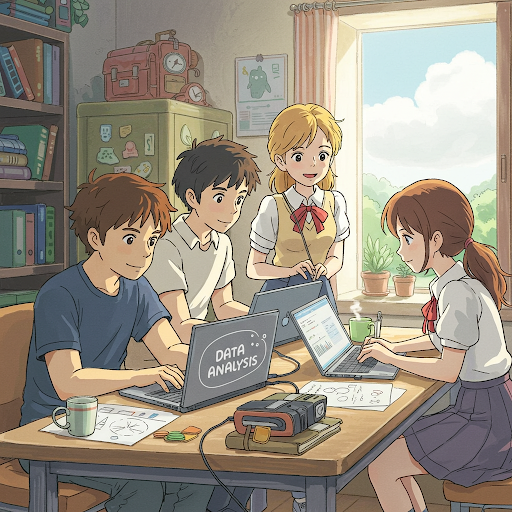
\includegraphics[width=8.5cm]{./figures/DAR.png}}
        \caption{Generated using \href{https://gemini.google.com/}{\myul{Gemini 2.5 Pro}} and the prompt:\\[4pt]
            \emph{Generate a group 4 of students working together on a project, brainstorming and collaborating.\\[4pt]
                They should have laptops. Add the text 'Data Analysis' on one screen. Make the image in cartoon style like Studio Ghibli}.}
        \vspace{-75pt}
        \label{fig:collaboration}
    \end{wrapfigure}
    This project relies heavily on effective teamwork and collaborative effort from everyone involved.

    To foster a positive and productive working environment, please ensure your group prioritises the following behaviours:
    \begin{itemize}
        \item \textbf{Clear and open communication:} Actively listen to each other and express ideas respectfully, ensuring everyone's voice can be heard.
        \item \textbf{Equitable task distribution:} Share responsibilities fairly amongst all team members, considering individual strengths and development goals where appropriate. Agree on roles and tasks collectively.
        \item \textbf{Regular team meetings:} Schedule and attend regular check-ins to discuss progress, address any challenges, and maintain alignment within the group organisation.
    \end{itemize}
    \vspace*{5mm}
    \textbf{Please bear in mind that}:
    \begin{itemize}
        \item All individuals in the group are expected to make significant contributions throughout every phase of the project. Active participation from everyone is essential for success.
        \item We strongly encourage you to explore different avenues, experiment with techniques, and apply creative thinking to your approach, whilst always basing your technical decisions on sound data analysis principles.
        \item The use of AI tools is permitted as an aid; however, transparency is required. Should you use such tools, please include comprehensive details regarding where, when, and how they assisted in the project's development (similar to the example provided in \Cref{fig:collaboration}).
    \end{itemize}

    \newpage
    \section{Acknowledgements}
    The data in this project has been acquired and curated by Eng. Jan Pinyol, under the supervision of Prof. Dr. Sergio Romero, and with help from MSc. Eng Oziel R. Cantú. Jan and Sergio have also contributed several figures and code examples.

    Profs. Dr. Alejandro Bachiller, Dr. Mónica Rojas, and Dr. Sergio Romero have also contributed with their experience in BCI and teaching in the HMI course, as well as reviewing this document.

    I also want to extend my gratitude to the volunteers at the \href{https://bioart.upc.edu}{\myul{BIOART Group}} for their selfless contribution to our EEG recording study.

    Thanks to you all!


    \begin{flushright}
        Joan F. Alonso\\
        Barcelona, April 2025
    \end{flushright}

    \newpage
    % --- Start Annexes ---
    \begin{appendices}
        % --- Appendix-specific formatting ---
        \titleformat{\section}
        {\color{upc}\normalfont\Large\bfseries\raggedright}
        {\color{upc}Annexe~\thesection} % Use British "Annexe"
        {1em}   % Separation
        {}      % Before code


        % --- Annexe sections ---
        \section{Description of the Database}
        \label{annex:database}

        The EEG data for this project were acquired using a 16-channel OpenBCI system, with the EEG signals referenced to the right mastoid.

        EEGLab was employed solely to read the data files generated by LabRecorder, allowing for the alignment of EEG data with temporal markers from the Psychopy experiment. No additional common referencing was performed in EEGLab (although the \texttt{.mat} files may indicate the contrary by default).

        \subsection{Channel Information}

        \begin{itemize}
            \item The channel labels in the \texttt{.mat} data files contain the raw output from the OpenBCI system (see \Cref{fig:OpenBCI}).
            \item Data transmission was managed via a command-line interface, which also facilitated the configuration of data transmission parameters, including amplifier gain. However, direct in-software renaming of channels is not currently supported by the OpenBCI software, nor the suppression of unused channels.
            \item The validated channel labels for analysis are, from 1 to 15: F7, F3, Fz, F4, F8, T3, C3, Cz, C4 , T4, P7, P3, Pz, P4, and P8. All of them correspond to the standars 10/20 international system.
            \item A 16th channel is present due to amplifier configuration and must be excluded from subsequent analysis.
        \end{itemize}

        \begin{figure}[htbp]
            \centering
            \Acrobatmenu{GoBack}{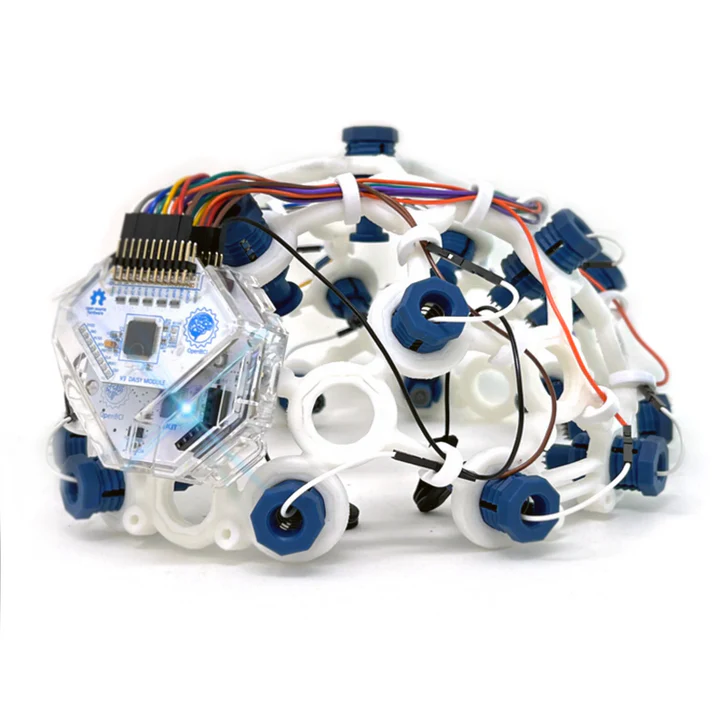
\includegraphics[trim=0cm 1cm 0cm 1cm, clip, width=9cm]{./figures/UCM4-003.png}}
            \caption{Ultracortex EEG headset and Cyton/Daisy bioamplifier. Image from the \href{https://shop.openbci.com/products/the-complete-headset-eeg?variant=44401726193904}{\myul{OpenBCI Shop}}.}
            \label{fig:OpenBCI}
        \end{figure}

        \subsection{Experimental Protocol}

        The experimental protocol involved \textbf{8 runs of 60 trials} each. Within each run, there were \textbf{20 trials of right-hand task}, \textbf{20 trials of left-hand task}, and \textbf{20 trials of rest}, which appeared in random order.

        The first \textbf{two runs consisted of motor executions (ME)}, while the remaining \textbf{six runs involved motor imagery (MI)}. This resulted in a total of 480 trials (8 runs $\times$ 60 trials), distributed as 160 trials for each condition (right-hand, left-hand, rest).

        Thus, for motor imagery (MI) classification, data start at the 121st trial. This subset comprises 360 MI trials (6 runs $\times$ 60 trials), with 120 trials per condition (right-hand, left-hand, rest).

        \subsection{Trial Structure}
        \begin{figure}[htbp]
            \centering
            \Acrobatmenu{GoBack}{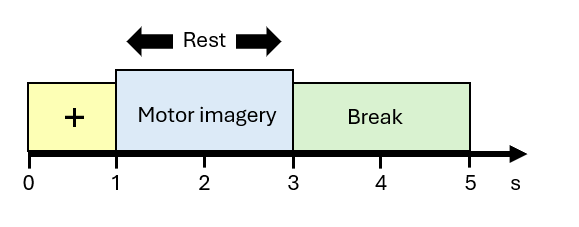
\includegraphics[width=8cm]{./figures/paradigm.png}} % Ensure figure path is correct
            \caption{Paradigm used in the motor imagery trials. Image by J. Pinyol.}
            \label{fig:paradigm}
        \end{figure}
        The experiment was programmed using PsychoPy. Each trial had an approximate duration of \SI{5}{\second} and followed this structure (see \Cref{fig:paradigm}): % British spelling programmed is correct
        \begin{itemize}
            \item \textbf{Fixation Cross:} \SI{5}{\second} + random duration in the range of $\pm\SI{0.2}{\second}$.
            \item \textbf{Task Period:} \SI{2}{\second}. Here the volunteer was shown either an arrow indicating right or left (for motor imagery), or the word \emph{Rest}.
            \item \textbf{Inter-Trial Interval:} \SI{2}{\second} + random duration in the range of $\pm\SI{0.2}{\second}$.
        \end{itemize}

        \clearpage
        \section{Project Report Rubric}
        \label{ann:projectrubric}
        % --- LaTeX Rubric for Report and Code Assessment ---
        \renewcommand{\arraystretch}{1.5}
        \scriptsize % Make text smaller to fit table
        \begin{longtable}{|>{\raggedright\arraybackslash}m{1.8cm}|>{\raggedright\arraybackslash}m{3.1cm}|>{\raggedright\arraybackslash}m{2.5cm}|>{\raggedright\arraybackslash}m{2.7cm}|>{\raggedright\arraybackslash}m{2.1cm}|>{\raggedright\arraybackslash}m{1.5cm}|c|}

            % --- Caption (Optional but Recommended) ---
            \caption{Project Report Rubric} \\

            % --- Header for First Page ---
            \hline
            \textbf{Aspect to Evaluate} & \textbf{Level 4\newline Outstanding} & \textbf{Level 3\newline Commendable} & \textbf{Level 2\newline Satisfactory} & \textbf{Level 1\newline Insufficient} & \textbf{Level 0\newline No Evidence} & \textbf{Weight} \\
            \hline \hline
            \endfirsthead % End of header for the first page

            % --- Header for Subsequent Pages ---
            \caption[]{Project Report Rubric (Continued)}\\ % Add Continued caption
            \hline
            \textbf{Aspect to Evaluate} & \textbf{Level 4\newline Outstanding} & \textbf{Level 3\newline Commendable} & \textbf{Level 2\newline Satisfactory} & \textbf{Level 1\newline Insufficient} & \textbf{Level 0\newline No Evidence} & \textbf{Weight} \\
            \hline \hline
            \endhead % End of header for subsequent pages

            % --- Footer (Optional, e.g., for page numbers or 'Continued on next page') ---
            \hline \multicolumn{7}{r}{{Continued on next page}} \\ \hline
            \endfoot % Footer for all pages except the last

            % --- Last Footer (Optional) ---
            \hline
            \endlastfoot % Footer only for the last page


            % --- Criterion 1 ---
            \textbf{1\newline\newline Introduction and Problem Description} &
            Provides a comprehensive and insightful introduction, clearly defining the problem, strong motivation, precise objectives, and a clear report outline. Context is exceptionally well-established. &
            Provides a clear introduction, defining the problem, motivation, objectives, and report outline. Context is well-established. &
            Provides a basic introduction, outlining the problem, motivation, objectives, and report structure. Some elements may lack detail or clarity. Context may be partially missing. &
            Introduction is unclear, incomplete, or significantly flawed. Problem, motivation, objectives, or structure are poorly defined or missing. &
            No introduction or problem description provided. &
            10\% \\ \hline

            % --- Criterion 2 ---
            \textbf{2\newline\newline Structure, Format, and Language} &
            Exceptionally well-organised report following all required sections. Professional formatting, excellent figures/tables integration. Language is precise, clear, concise, and error-free academic English. & % Corrected organised
            Well-organised report adhering to structure. Good formatting and integration of visuals. Language is clear, mostly concise, and uses appropriate academic English with minimal errors. & % Corrected organised
            Generally organised report, most sections present. Formatting is adequate but may have inconsistencies. Language is understandable but may lack conciseness or contain several errors. & % Corrected organised
            Poorly organised, sections missing or illogical. Formatting is inconsistent or unprofessional. Language is unclear, verbose, or contains significant errors. & % Corrected organised
            Report structure/ format makes it unreadable or unevaluable. &
            15\% \\ \hline

            % --- Criterion 3 ---
            \textbf{3\newline\newline Methodology and Tool Usage (MATLAB,\newline Python)} &
            Detailed, clear, and well-justified description of all steps (data description, preprocessing, feature engineering/ selection, model choice, validation strategy). Excellent and appropriate use of MATLAB/Python demonstrated. &
            Clear description and justification of most methodological steps. Appropriate use of MATLAB/Python for the required tasks demonstrated. &
            Basic description of methodology, some justifications may be weak or missing. Adequate use of MATLAB/Python, but perhaps not fully leveraged or with minor issues. &
            Methodology is poorly described, illogical, or inappropriate for the problem. Tools (MATLAB/Python) are used incorrectly or insufficiently. &
            No methodology described or tool usage shown. &
            15\% \\ \hline

            % --- Criterion 4 ---
            \textbf{4\newline\newline Results: Metrics and Visualisations} & % British spelling Visualisations
            Presents comprehensive and insightful results using highly relevant metrics. Figures/tables are exceptionally clear, well-labelled, informative, perfectly integrated, and expertly explained in the text. & % Corrected labelled
            Presents clear results using appropriate metrics. Figures/tables are clear, well-labelled, adequately integrated, and well-explained in the text. & % Corrected labelled
            Presents basic results, some relevant metrics might be missing. Figures/tables are present but may lack clarity, labels, or sufficient explanation/ integration in the text. & % Corrected labels
            Results are unclear, irrelevant, or poorly presented. Metrics are inappropriate or missing. Figures/tables are confusing, poorly labelled, or absent. & % Corrected labelled
            No results presented. &
            15\% \\ \hline

            % --- Criterion 5 ---
            \textbf{5\newline\newline Discussion and Critical Interpretation} &
            Provides insightful and deep interpretation of results, critically analysing strengths/weaknesses. Effectively relates findings to objectives and BCI context. Discusses implications and limitations thoroughly. & % Corrected analysing
            Provides clear interpretation of results, analysing strengths/weaknesses. Relates findings to objectives and context well. Discusses implications and limitations adequately. & % Corrected analysing
            Provides basic interpretation of results. Some analysis of strengths/weaknesses present. Connection to objectives/context is made but may be superficial. Basic discussion of limitations. & % British spelling analysis (noun) is correct
            Interpretation is minimal, incorrect, or superficial. Little to no analysis of strengths/weaknesses or connection to objectives/context. & % British spelling analysis (noun) is correct
            No discussion or interpretation provided. &
            15\% \\ \hline

            % --- Criterion 6 ---
            \textbf{6\newline\newline Conclusions and Originality} &
            Draws strong, well-supported conclusions directly addressing all objectives. Offers significant original insights, novel approaches, or critical reflections beyond the baseline requirements. &
            Draws clear conclusions addressing the main objectives. May offer some original insights or thoughtful reflections on the process or results. &
            Draws basic conclusions related to objectives, but may lack depth or full support from results. Limited evidence of original thought or reflection. &
            Conclusions are weak, unsupported, irrelevant, or missing. No evidence of originality or critical reflection. &
            No conclusions provided. &
            15\% \\ \hline

            % --- Criterion 7 ---
            \textbf{7\newline\newline Code: Clarity,\newline Comments,\newline and\newline Functionality} &
            Code is exceptionally clear, well-structured, efficiently written, and thoroughly documented (comments, README). It runs flawlessly and reproduces the results described. Best practices are followed. &
            Code is clear, reasonably structured, and adequately documented. It runs correctly and reproduces the main results. Good practices are generally followed. &
            Code is generally understandable but may lack structure or sufficient documentation. It runs but may require minor fixes or clarifications to reproduce results. Basic coding practices followed. &
            Code is difficult to understand, poorly structured, or lacks documentation. It fails to run correctly or reproduce results without significant effort. &
            No code submitted, or code is completely non-functional. &
            15\% \\ \hline
        \end{longtable}

        \newpage % Start presentation rubric on a new page
        \section{Presentation Rubric}
        \label{ann:presentationrubric}
        \renewcommand{\arraystretch}{1.5}
        \scriptsize % Make text smaller to fit table
        \begin{longtable}{|>{\raggedright\arraybackslash}m{1.8cm}|>{\raggedright\arraybackslash}m{3.1cm}|>{\raggedright\arraybackslash}m{2.5cm}|>{\raggedright\arraybackslash}m{2.7cm}|>{\raggedright\arraybackslash}m{2.1cm}|>{\raggedright\arraybackslash}m{1.5cm}|c|}
             \caption{Presentation Rubric} \\
            \hline
            \textbf{Aspect to Evaluate} & \textbf{Level 4\newline Outstanding} & \textbf{Level 3\newline Commendable} & \textbf{Level 2\newline Satisfactory} & \textbf{Level 1\newline Insufficient} & \textbf{Level 0\newline No Evidence} & \textbf{Weight} \\
            \hline \hline

            % --- Criterion 1 ---
            \textbf{1\newline\newline Organisation and Structure} & % Corrected Organisation
            Exceptionally clear and logical flow. Introduction perfectly sets the stage (context, objectives), and conclusion provides a strong, insightful summary. Transitions are seamless. &
            Clear and logical flow. Introduction effectively presents context and objectives. Conclusion summarises key points well. Transitions are smooth. & % Corrected summarises
            Generally logical flow, but some parts may be slightly disorganised. Introduction and conclusion cover basic points but could be clearer or more impactful. Transitions are adequate. & % Corrected disorganised
            Disorganised flow, difficult to follow. Introduction or conclusion are weak, missing key elements, or unclear. Transitions are abrupt or confusing. & % Corrected Disorganised
            No discernible organisation or structure. & % Corrected organisation
            15\% \\ \hline

            % --- Criterion 2 ---
            \textbf{2\newline\newline Content Clarity and Depth} &
            Explanations of problem, methods, results, and significance are exceptionally clear, accurate, and demonstrate deep understanding. Insightful connections made. &
            Explanations are clear, accurate, and demonstrate a good understanding of the project concepts and details. &
            Explanations are generally understandable but may lack some clarity or depth. Basic understanding demonstrated. &
            Explanations are unclear, inaccurate, or superficial. Demonstrates poor understanding of the project content. &
            Content is irrelevant or incomprehensible. &
            25\% \\ \hline

            % --- Criterion 3 ---
            \textbf{3\newline\newline Visual Aids and Delivery} &
            Visual aids are highly professional, informative, and perfectly support the talk. Delivery is engaging, clear, well-paced, and demonstrates confidence. Excellent use of language. &
            Visual aids are clear, relevant, and effectively used. Delivery is clear, well-paced, and confident. Good use of language. &
            Visual aids are adequate but may have minor issues (e.g., clutter, relevance). Delivery is generally clear but may lack engagement or have minor flaws (pace, clarity). &
            Visual aids are poor quality, confusing, or used ineffectively. Delivery is unclear, hesitant, poorly paced, or lacks engagement. &
            No visual aids used, or delivery prevents understanding. &
            20\% \\ \hline

            % --- Criterion 4 ---
            \textbf{4\newline\newline Teamwork and Time Management} &
            Excellent coordination, seamless transitions, and clearly balanced participation. Presentation perfectly fits the allocated time. &
            Good coordination, smooth transitions, and balanced participation among group members. Presentation adheres well to the time limit. &
            Adequate coordination and participation, though some imbalance or minor issues with transitions may exist. Generally adheres to time limit, may be slightly over/under. &
            Poor coordination, awkward transitions, or significantly unbalanced participation. Poor adherence to time limits (significantly over/under). &
            No evidence of teamwork, or time management hinders presentation. &
            10\% \\ \hline

            % --- Criterion 5 ---
            \textbf{5\newline\newline Answering Questions} &
            Demonstrates mastery by providing exceptionally clear, accurate, concise, and insightful answers to all questions. Handles challenging questions effectively. &
            Provides clear, accurate, and thoughtful answers to questions, demonstrating a solid understanding of the project. Handles most questions well. &
            Provides generally adequate answers, but some may lack clarity, depth, or accuracy. Demonstrates basic understanding but struggles with complex questions. &
            Unable to answer most questions accurately or clearly. Responses are confused, incorrect, or demonstrate a lack of understanding. &
            Does not attempt to answer questions or responses are irrelevant. &
            30\% \\ \hline

        \end{longtable}

    \end{appendices}

\end{document}